\begin{figure}[htpb]
    \centering
    \begin{subfigure}[b]{0.475\textwidth}
        \centering
        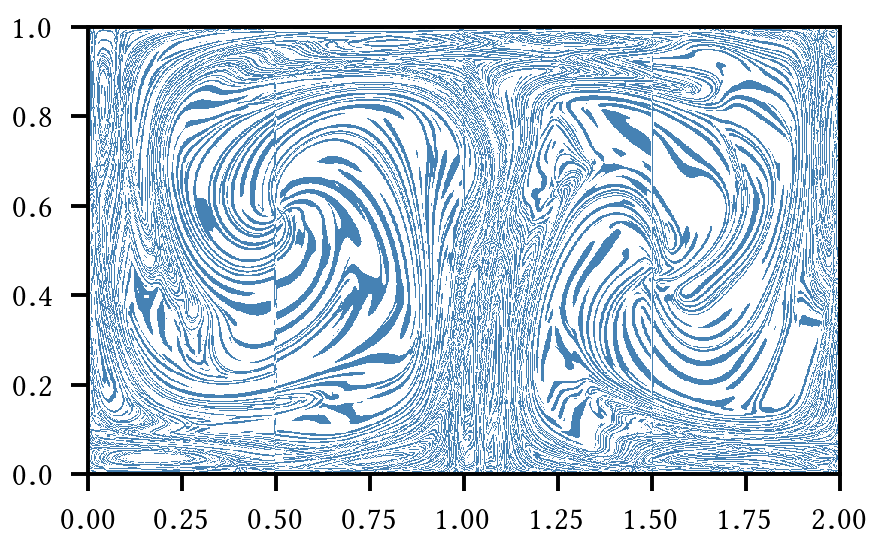
\includegraphics{figures/domain_figures/rkbs32_err_half_width.png}
        \caption[]{{\small Bogacki-Shampine 3(2)}}
        \label{fig:u0_dom_err_bs32}
    \end{subfigure}
    \begin{subfigure}[b]{0.475\textwidth}
        \centering
        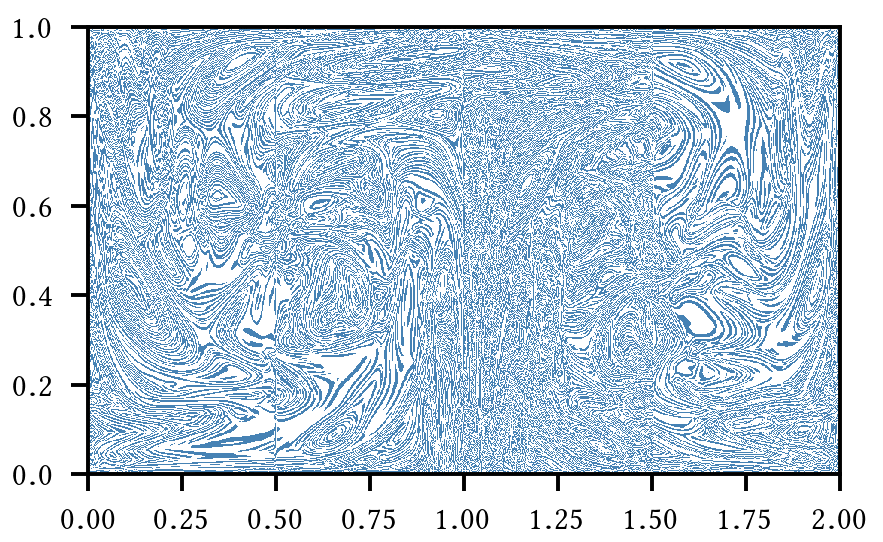
\includegraphics{figures/domain_figures/rkbs54_err_half_width.png}
        \caption[]{{\small Bogacki-Shampine 5(4)}}
        \label{fig:u0_dom_err_bs54}
    \end{subfigure}

    \begin{subfigure}[b]{0.475\textwidth}
        \centering
        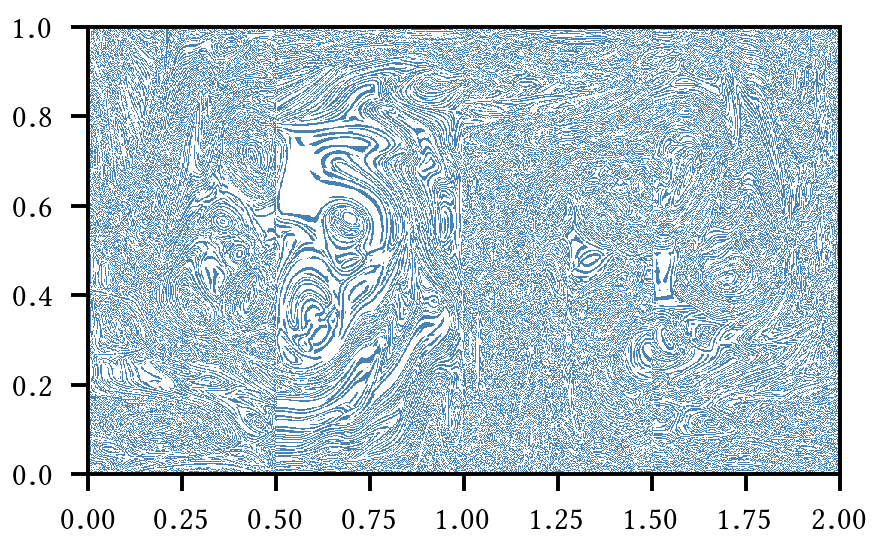
\includegraphics{figures/domain_figures/rkdp54_err_half_width.png}
        \caption[]{{\small Dormand-Prince 5(4)}}
        \label{fig:u0_dom_err_dp54}
    \end{subfigure}
    \begin{subfigure}[b]{0.475\textwidth}
        \centering
        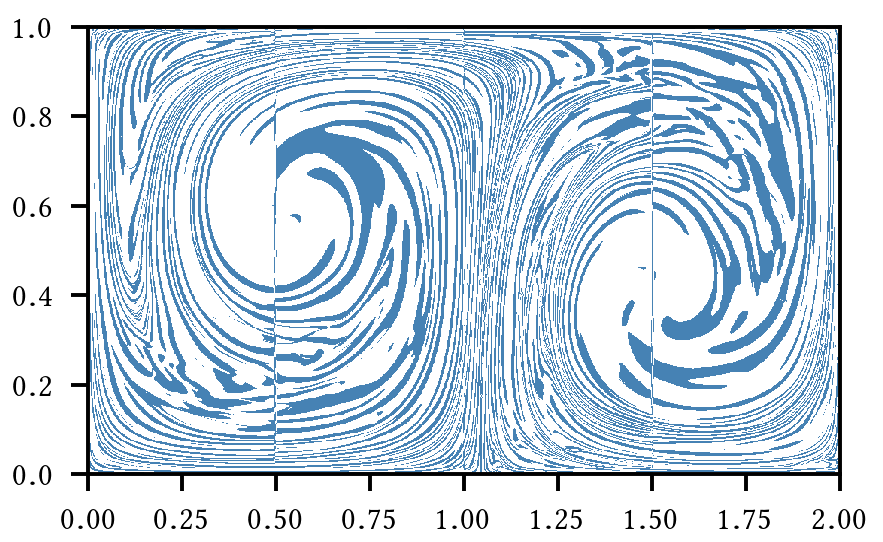
\includegraphics{figures/domain_figures/rkdp87_err_half_width.png}
        \caption[]{{\small Dormand-Prince 8(7)}}
        \label{fig:u0_dom_err_dp87}
    \end{subfigure}
    \caption[The $\mathcal{U}_{0}$ domains obtained with the adaptive stepsize
    integration schemes, with numerical tolerance level
    $\textnormal{tol}=10^{-1}$]{
        The $\mathcal{U}_{0}$ domains obtained with the adaptive stepsize
        integration schemes, with numerical tolerance level
        $\textnormal{tol}=10^{-1}$. Out of the four schemes considered, only the
    Dormand-Prince 8(7) method is remotely close to reproducing the
    reference domain, shown in~\ref{fig:u0_domain}. In any case, the
    differences are sufficiently large to alter the resulting strain
    system beyond recognition, rendering LCS comparisons with the reference
    impractical.}
    \label{fig:u0_dom_errs}
\end{figure}

